%=============================================================
\chapter{System Design}
\label{ch:arch}
%=============================================================

PaceANN is a disk-based search layer that can be applied directly to existing DiskANN indexes.
It preserves the original index layout and changes only the search path.
As shown in Figure~\ref{fig:overview}, each search hop first checks whether the query has converged through Convergence-Aware Early Termination (CA-ET).
If the query continues, the search consults the Popularity-Adaptive Cache Manager (PAC).
A cache hit serves the neighbor list and full-precision vector from DRAM; a miss falls back to the original SSD read path.

\begin{figure}[htbp]
  \centering
  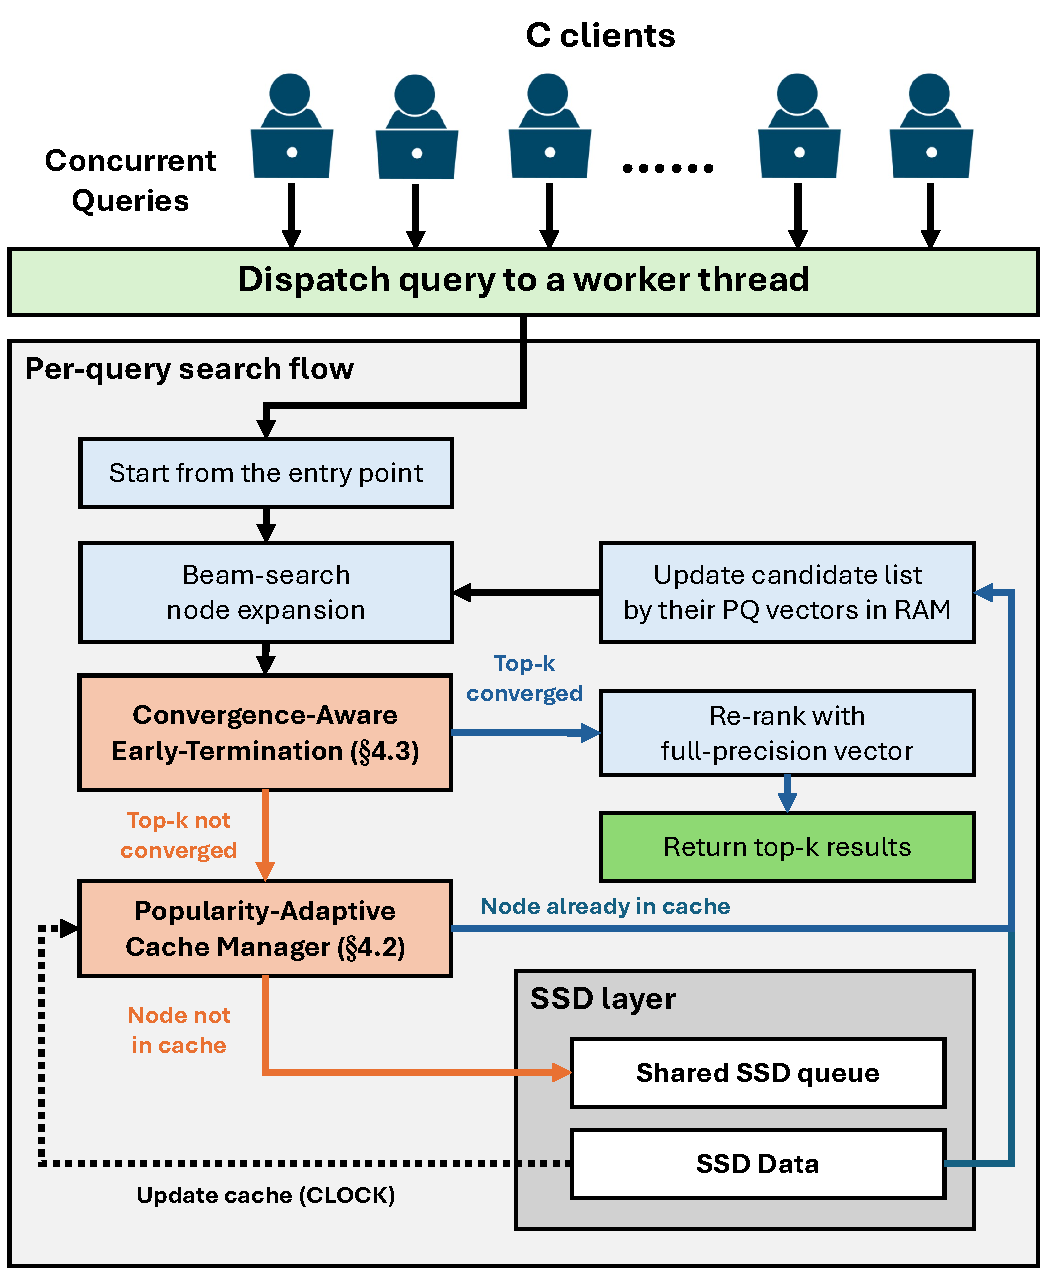
\includegraphics[width=0.6\textwidth]{img/paceann_overview.pdf}
  \caption[Overview of PaceANN]{Overview of PaceANN. Concurrent queries are processed by a server-side worker-thread pool. Before each hop, CA-ET decides whether the query has converged. If not, PAC is consulted. Cache hits return the neighbor list and full-precision vector from DRAM for both traversal and re-ranking; misses fall back to the shared SSD queue.}
  \label{fig:overview}
\end{figure}

PAC and CA-ET are designed to work together.
PAC reduces the cost of useful hops and provides exact vectors for convergence checks.
CA-ET removes later expansions after the query has converged.
Together, they reduce the number of random reads entering the shared SSD queue.

%-------------------------------------------------------------
\section{Popularity-Adaptive Cache Manager (PAC)}
\label{sec:cache}
%-------------------------------------------------------------

PAC caches graph nodes that are likely to be visited repeatedly.
It starts with a small cold-start seed built by BFS from the DiskANN medoid, because early search hops repeatedly pass through the entry neighborhood.
After startup, PAC is demand-filled: when a node is read from SSD, it can be inserted into the cache.
This lets the cache adapt to the actual query distribution instead of relying only on a static BFS cache or a separate warm-up workload.

The cache is sharded to support concurrent serving.
With $T$ worker threads, PAC uses $S = 2^{\lceil \log_2 T \rceil}$ shards; in our experiments, $T=32$ and $S=32$.
Shard selection uses the bit mask \texttt{node\_id \& (S$-$1)}.
Each shard maintains a hash table and a CLOCK replacement ring protected by a \texttt{shared\_mutex}.
Lookups use shared locks and only update a small atomic reference counter.
Insertions use non-blocking \texttt{try\_lock}; if the shard is busy, the insertion is skipped rather than delaying the query.
CLOCK replacement gives recently used entries a second chance while avoiding the per-hit exclusive updates required by exact LRU\cite{corbato1968clock,megiddo2003arc}.

Each PAC entry stores both the neighbor list and the raw full-precision vector.
This coordinate co-storage is important because DiskANN normally performs traversal using neighbor IDs and PQ distances, then fetches full vectors again for re-ranking.
When a node hits in PAC, both traversal and re-ranking can be served from DRAM, so the hit avoids SSD I/O across the full query path.
The cost is a larger cache entry, which is included in the memory budget.

\begin{figure}[htbp]
  \centering
  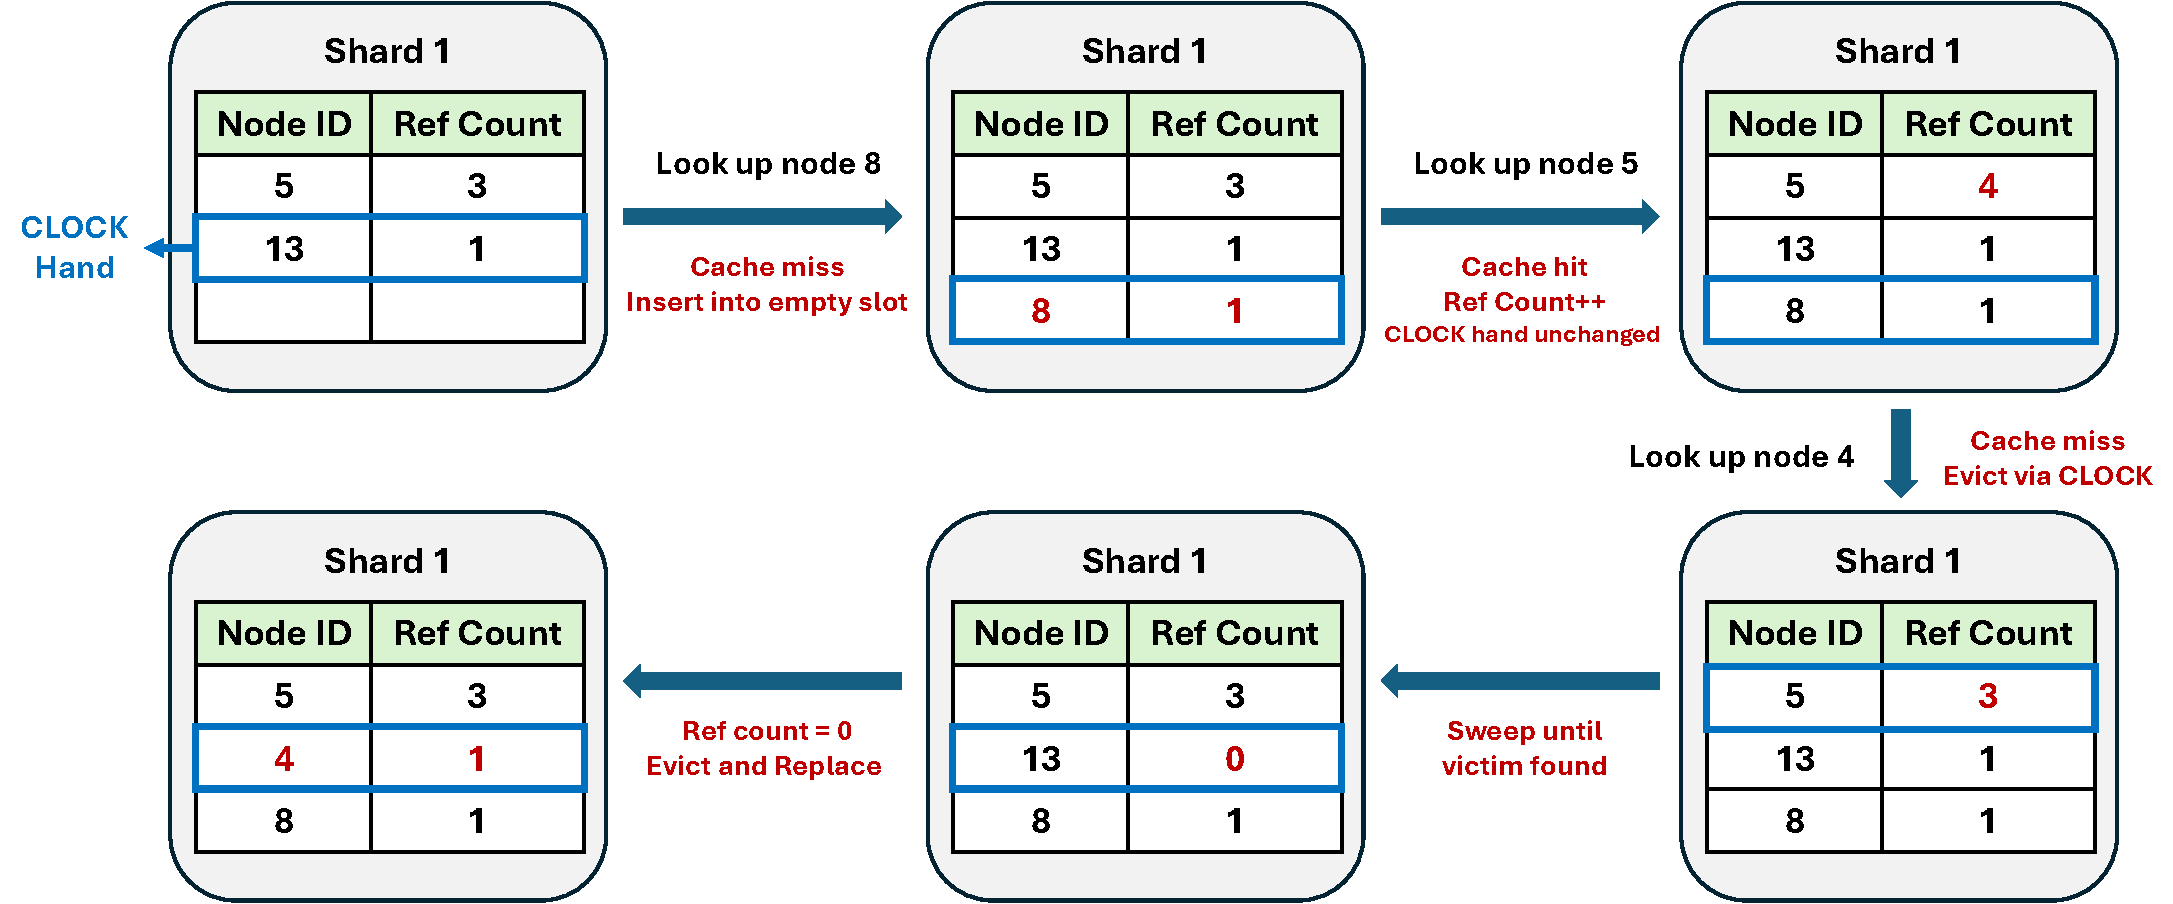
\includegraphics[width=1\textwidth]{img/cache_showcase.pdf}
  \caption[Popularity-Adaptive Cache Manager]{Popularity-Adaptive Cache Manager (PAC). Nodes are assigned to shards using \texttt{node\_id \& (S$-$1)}. Each slot co-stores the neighbor list and the full-precision vector. A cache hit serves both traversal and re-ranking from DRAM; a miss issues an SSD read and inserts the returned neighbor list and coordinates if the shard lock is available. Lookups use shared locks, while insertions use non-blocking \texttt{try\_lock}.}
  \label{fig:bnc}
\end{figure}

%-------------------------------------------------------------
\section{Convergence-Aware Early Termination (CA-ET)}
\label{sec:et}
%-------------------------------------------------------------

CA-ET adds a stopping rule inside DiskANN beam search.
Before each expansion, PaceANN selects the unexpanded candidate with the smallest PQ-estimated distance, denoted $v_\text{best\text{-}unexp}$.
It compares this estimate with the exact distance of the current $2k$-th candidate:

\begin{equation}
  d_\text{PQ}(q,\, v_\text{best\text{-}unexp}) \;>\; \theta \cdot d_\text{exact}(q,\, v_{2k})
  \label{eq:et-gate}
\end{equation}

If the condition holds, the best remaining frontier candidate is unlikely to improve the current top-$k$ result, so the search can stop.
The rule uses PQ distance on the frontier side because those codes are already in memory, and exact distance on the result side because expanded candidates have already fetched their full vectors.
Therefore, the stopping check does not issue any additional SSD reads.

The threshold $\theta$ controls aggressiveness.
Smaller values stop earlier but risk recall loss; larger values are more conservative and approach baseline DiskANN behavior.
Because PQ distance is approximate rather than a true lower bound, PaceANN also uses two safeguards: a patience counter requiring the condition to hold for $P$ consecutive hops, and a minimum-hop threshold $t_\text{min}$ that disables early termination during the unstable beginning of search.

%-------------------------------------------------------------
\section{Why Caching and Early Termination Must Be Co-designed}
\label{sec:codesign}
%-------------------------------------------------------------

Caching alone reduces some SSD reads, but it does not reduce the number of beam-search hops.
Post-convergence hops can still consume DRAM bandwidth, lock operations, and CPU time even when they hit in cache.
Early termination alone also has a weakness: without cached early hops, the current top-$k$ boundary is less stable, so the stopping rule must be conservative to avoid recall loss.

When both mechanisms are enabled, PAC helps the early search state stabilize quickly and provides exact vectors for CA-ET.
CA-ET then removes the remaining post-convergence work.
The combined effect is a lower SSD read arrival rate, which reduces queue depth and improves throughput and tail latency under high concurrency.

%-------------------------------------------------------------
\section{Concurrent Serving Architecture}
\label{sec:server}
%-------------------------------------------------------------

The PaceANN server uses a fixed worker-thread pool.
Each worker keeps thread-local per-query state such as the retset and visited bitmap.
After receiving a query, a worker runs the full search and returns the result.
This same client/server measurement framework is used for all evaluated systems, while each system keeps its native server-side I/O implementation.
